% --------------------------------------------------------------------------- %
%                   __                      _                                 %
%  _ __   ___ _ __ / _| ___  _ __ _ __ ___ (_)_ __   __ _                     %
% | '_ \ / _ \ '__| |_ / _ \| '__| '_ ` _ \| | '_ \ / _` |                    %
% | |_) |  __/ |  |  _| (_) | |  | | | | | | | | | | (_| |                    %
% | .__/ \___|_|  |_|  \___/|_|  |_| |_| |_|_|_| |_|\__, |                    %
% |_|                                               |___/                     %
%                                         _                                   %
%                             _ __   ___ | |_   _  __ _  ___  _ __  ___       %
%                            | '_ \ / _ \| | | | |/ _` |/ _ \| '_ \/ __| /\/| %
%                            | |_) | (_) | | |_| | (_| | (_) | | | \__ \|/\/  %
%                            | .__/ \___/|_|\__, |\__, |\___/|_| |_|___/      %
%                            |_|            |___/ |___/                       %
% --------------------------------------------------------------------------- %
\chapter{Performing polygons\textasciitilde{}}\label{sec: polygons}
\begin{flushright}
    \Large\textsc{Developing a Sound ARt Performance Practice}
\end{flushright}
%\markboth{}{Performing polygons\textasciitilde{}
\begin{SingleSpace}
    \noindent \textbf{polygons\textasciitilde{} Blog:}        \url{https://www.sambilbow.com/projects/polygons}

    \noindent \textbf{polygons\textasciitilde{} Code:}        \url{https://www.github.com/sambilbow/polygons}

    \noindent \textbf{polygons\textasciitilde{} Guide:}       \url{https://www.github.com/sambilbow/polygons/wiki}
\end{SingleSpace}

\begin{figure}
    \centering
    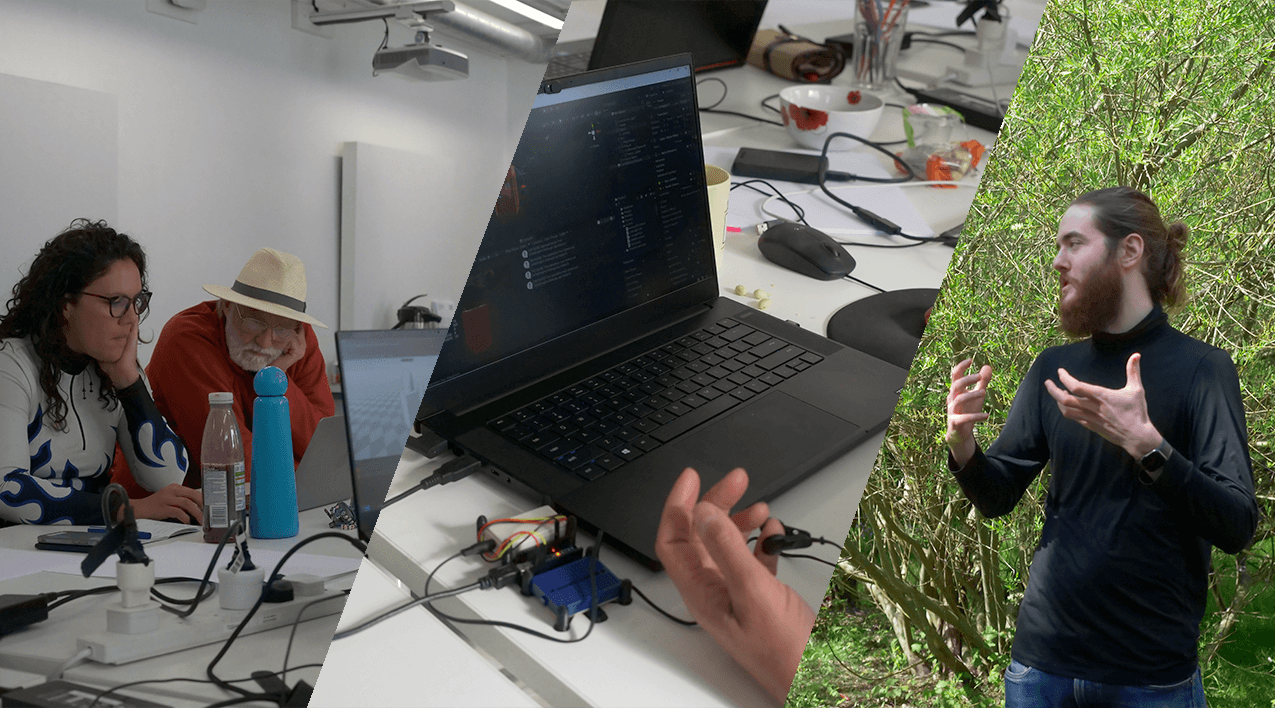
\includegraphics[width=1\linewidth]{07-polygons/chapter-fig.png}
    \captionsetup{labelformat=empty}
    \caption[\autoref{sec: polygons}: \textit{polygons\textasciitilde{}} in performance at The Rosehill, Brighton, 19th February, (from \citeauthor{bilbow2022b}, \citeyear{bilbow2022b})]{}
\end{figure}

\clearpage
% --------------------------------------------------------------------------- %
\section{Summary}\label{sec: polygons-developing}
As a direct consequence of witnessing participants enjoyment and play with \textit{polaris\textasciitilde{}}, I recognised for the first time looking from the outside in, that the system had a larger propensity for fostering learning, virtuosity, and depth of expression than I had originally thought; if only the experience was slightly more complex, the interactions more \textit{nuanced}. The gestures, play, and expression by participants led to a kind of quasi-transhumanist dance, one that struck me as a technologically mediated dialogue between hybrid self and hybrid environment, a delicate balance of agency.



Until this point, I had been primarily focused on the medium as used for the composition of musical pieces e.g. \hyperref[sec: area]{\textit{area\textasciitilde{}}}, or of installation-like experiences \hyperref[sec: polaris]{\textit{polaris\textasciitilde{}}}. Performance with AR had remained abstract, especially as, formally, its not my preferred mode of musical expression. However, the balance of agency between participant and system, between self and environment, presented itself during the evaluation of \textit{polaris\textasciitilde{}} to be an area ready for exploration through performance. 

The following chapter outlines my exploration of a a fifteen-minute experimental audiovisual AR improvisation using an AR performance ecosystem called \textit{Weird Polygons and Hand Noises}, or \textit{polygons\textasciitilde{}} for short.



% --------------------------------------------------------------------------- %
\section{The Composition of \textit{polygons\textasciitilde{}}}\label{sec: polygons-composition}

%*[ ]   What?
Drawing from the categories extracted from \nameref{sec: polaris}: \nameref{sec: polaris-feedback}, I pursued the design of a system with physically moveable elements, audio-reactivity, and enough room to be able to learn and explore the scene both spatially and in terms of interaction and sonic palette. Thus, as an AR performance ecosystem, \textit{polygons\textasciitilde{}} delivers this by describing the improvisational and performative relationship between a performers actions via body, hand, and head movement, feedback from the audience, and three real-time AR musical instruments: \textit{ambi}, \textit{click}, and \textit{hands}. 

%*[ ]   add unity image of ambi w/ particles
\textit{ambi}, a red wire-frame icosahedron, serves as a dual-oscillator drone synthesiser that the performer can call on my taking and bringing it closer to them with their hands. Its voice is contingent eleven real-time parameters, which are sent to the PureData patch attached to it. At specified distance two particle systems are activated from the palms of the performers hands, and the drone from \textit{ambi} is activated. The particles are drawn to the centre of \textit{ambi}, their paths guided by an unseen particle forcefield - the same behaviour as in \textit{polaris\textasciitilde{}}. Real-time hand `collision' in three dimensions with \textit{ambi} is constantly reported per hand, resulting in two sets of $x,y,z$ coordinates that form part of the data that is mapped to parameters in PureData (see \autoref{fig: polygons-ambi-mapping}).
\begin{table}
    \centering
    \begin{tabular}{ l|l l }
        \textbf{Unity Scene Attribute}  & \multicolumn{2}{ l }{\textbf{PureData Parameter}}   \\
        \hline
        \textbf{Hand}                   & \textbf{via Left Hand}& \textbf{via Right Hand}       \\
        \hline
        Collision Distance              & Drone 1 On / Off      & Drone 2 On / Off              \\
        Collision X                     & Reverb Amount         & Drone 2 LPF CF Mod            \\
        Collision Y                     & Drone 1 Pitch         & Drone 2 Pitch                 \\
        Collision Z                     & Rev/Dly Amount        & Drone 2 LPF CF                \\
        \hline
        
        \textbf{\textit{ambi}}          & \multicolumn{2}{ l }{\textbf{via pinch gesture}}    \\
        \hline
        Scale                           & \multicolumn{2}{ l }{Output Filter Cutoff}          \\  
    \end{tabular}
    \caption{The parameter mappings for \textit{ambi}}
    \label{fig: polygons-ambi-mapping}
\end{table}
%*[ ]   move panel in patch under each other for space
\begin{figure}
    \centering
    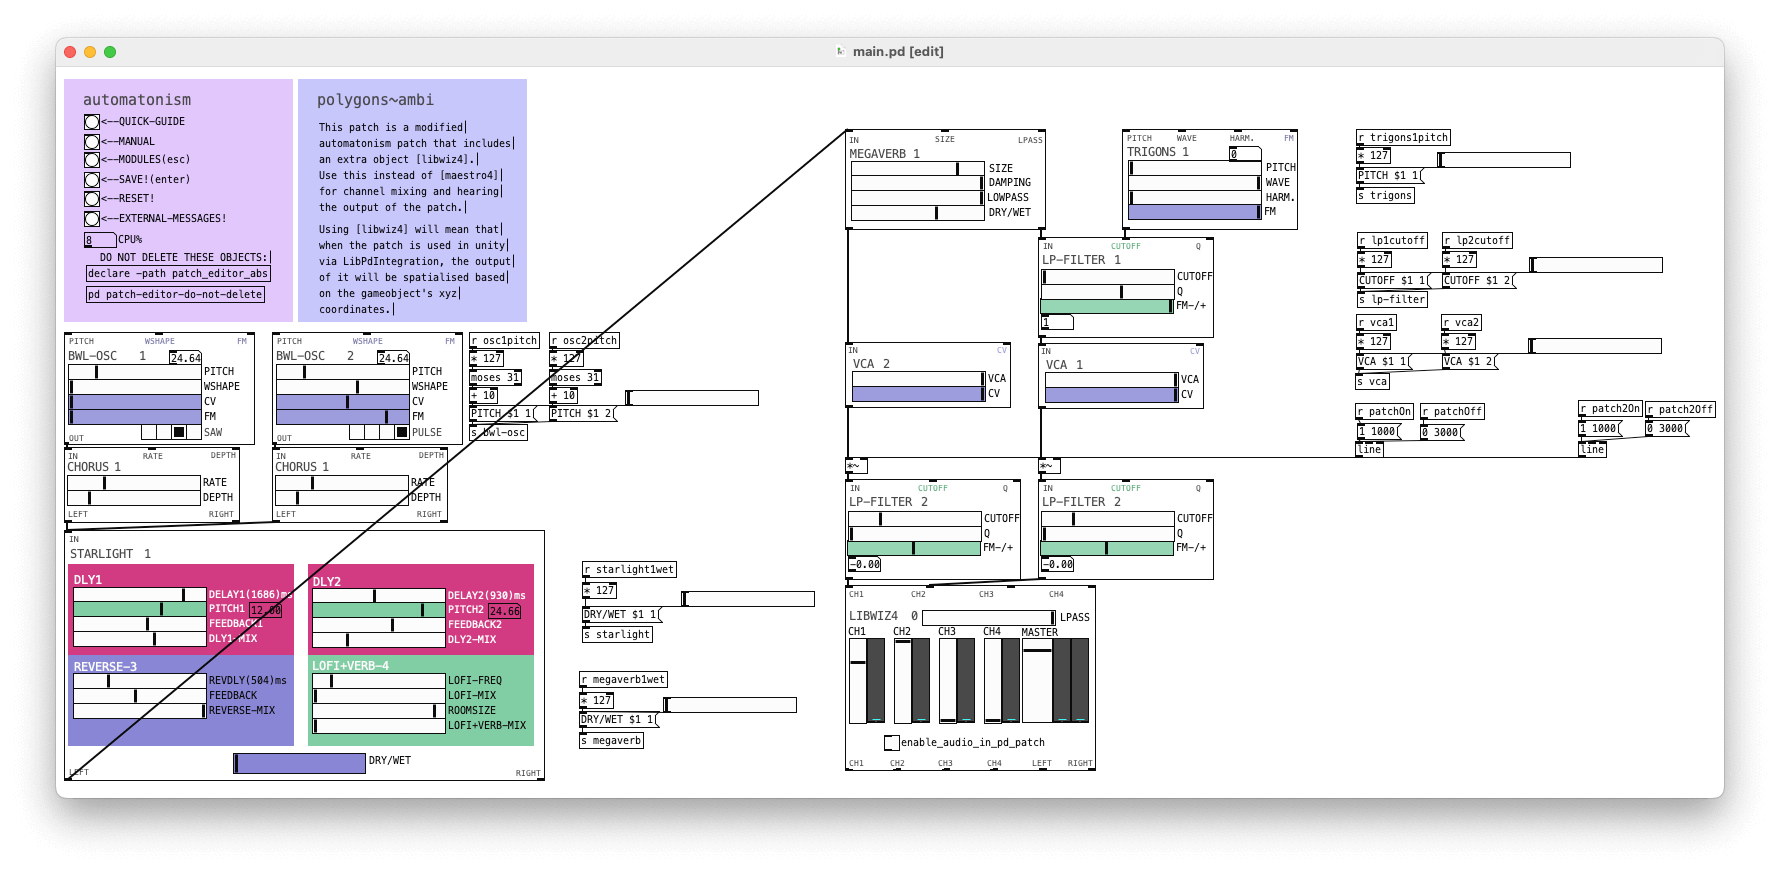
\includegraphics[angle=90,height=0.9\textheight]{07-polygons/polygons-ambi-pd.png}
    \caption{The PureData patch for \textit{ambi}}
    \label{fig: polygons-ambi-pd}
\end{figure}

%*[ ]   add unity image of click w/ particles
\textit{click}, a set of two blue wire-frame icosahedra, form a feedback system between two low-frequency oscillator controlled impulse generators. The feedback can be altered by bringing the smaller icosahedron (\textit{click-}) closer to the larger one (\textit{click+}). \textit{click+-} makes use of LibPdIntegration's Unity send functionality; each time there is an impulse generated, a message is sent to Unity, which triggers a shower of particles to be emitted from \textit{click-} to \textit{click+} forcefield-guided cone. As the performer intervenes and creates the feedback system, the closer they bring the icosahedra together, the faster the visual particle shower becomes, and the more erratic the impulse generators feedback on each other. A further sound parameter, connected to a reverb, is mapped to the amount spin \textit{click-} let go with by the performer. The sound palette explores a gradient from static electricity crackles to a sound akin toa car motor catching and revving up as the feedback increases.
\begin{table}
    \centering
    \begin{tabular}{ l|l }
        \textbf{Unity Scene Attribute}         & \textbf{PureData Parameter}   \\
        \hline      
        \textit{click+-} Distance              & Impulse 1 Frequency           \\
        \textit{click-} Collision X            & Impulse 2 Frequency           \\
        \textit{click-} Collision Y            & Impulse Chorus Rate           \\
        \textit{click-} Collision Z            & Impulse Chorus Depth          \\
        \textit{click-} Release Spin Velocity  & Impulse Reverb Amount     
    \end{tabular}
    \caption{The parameter mappings for \textit{click}}
    \label{fig: polygons-click-mapping}
\end{table}
\begin{figure}
    \centering
    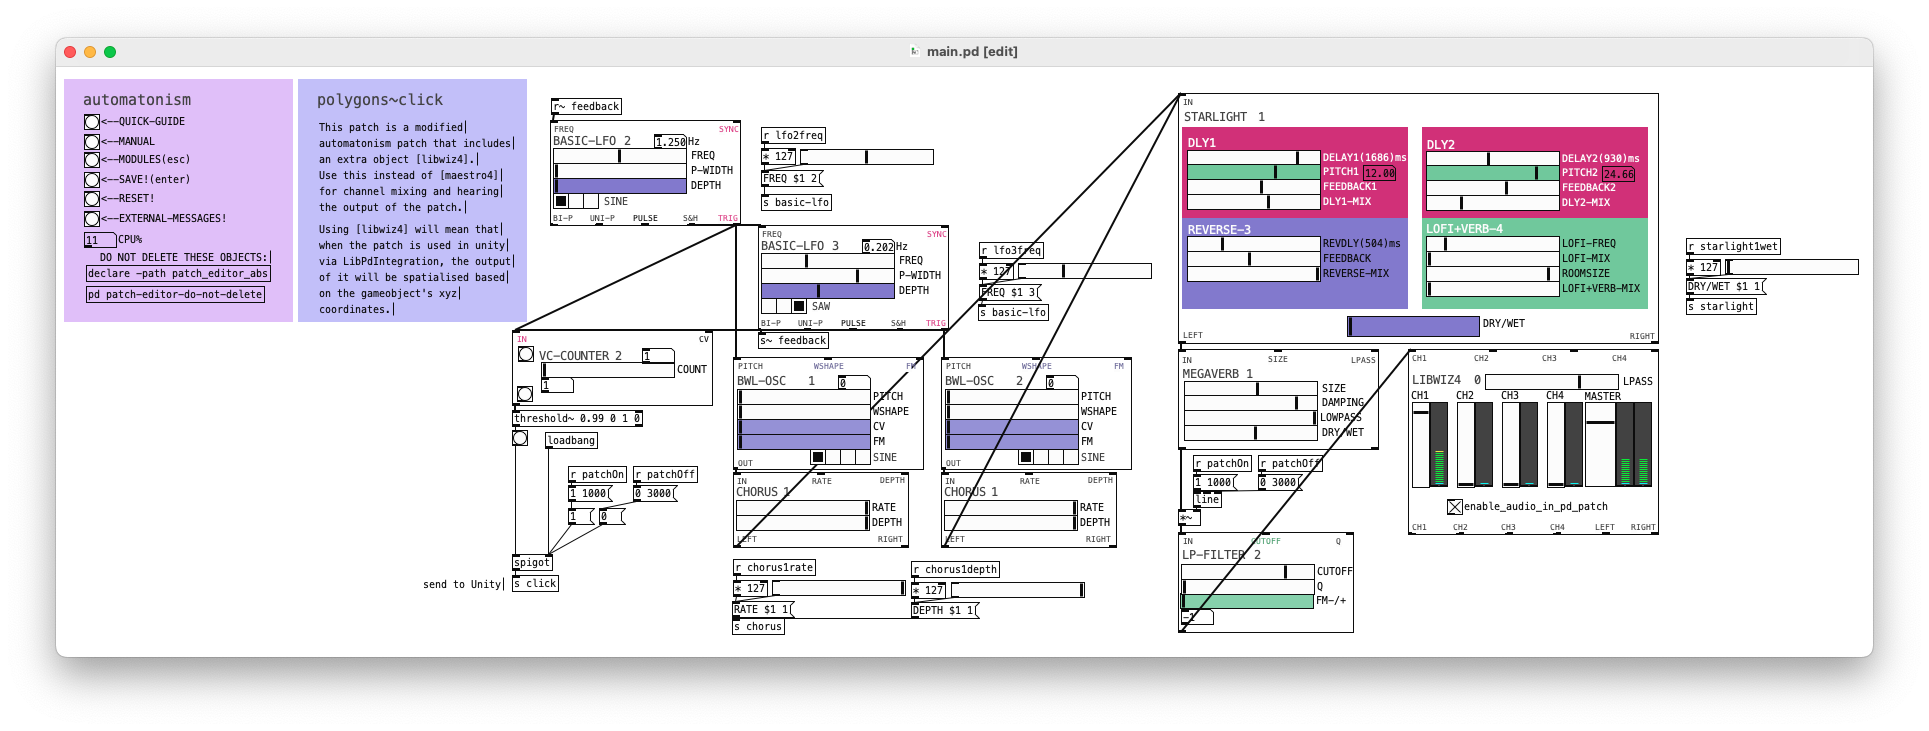
\includegraphics[angle=90,height=0.9\textheight]{07-polygons/polygons-click-pd.png}
    \caption{The PureData patch for \textit{click}}
    \label{fig: polygons-click-pd}
\end{figure}

%*[ ]   add unity image of hand w/ colours
\textit{hands} constitutes the final AR instrument in \textit{polygons~}; each of the performers hands, when a virtual button besides their palm is toggled \textit{on}, generate a highly resonant filtered white noise. The cutoff, resonance, and amplitude of this generator-filter system is controllable independently per hand, through several dynamic movement-based attributes. The filter cutoff per hand is mapped to that hand's distance to the performer's face; the filter resonance per hand is mapped to the angle from that hand's palm angle towards the centre of the performance space; and the amplitude of each is mapped to the stretching of the fingers outwards away from the palm. The sounds delivered by \textit{hands} are harsh and unpleasant at certain parameter combinations and purposefully loud; from a performative standpoint, this engenders specific gestures, movements, and stances, as the performer grapples with a sonic experience akin to howling and shrieking winds.
\begin{table}
    \centering
    \begin{tabular}{ l|l }
        \textbf{Unity Scene Attribute}         & \textbf{PureData Parameter}    \\
        \hline      
        \textit{hand} to Head Distance         & Filter Cutoff                  \\
        \textit{hand} to Stage Angle           & Filter Resonance               \\
        \textit{hand}'s Finger Extension       & Amplitude               
    \end{tabular}
    \caption{The parameter mappings for \textit{hands}}
    \label{fig: polygons-hands-mapping}
\end{table}
\begin{figure}
    \centering
    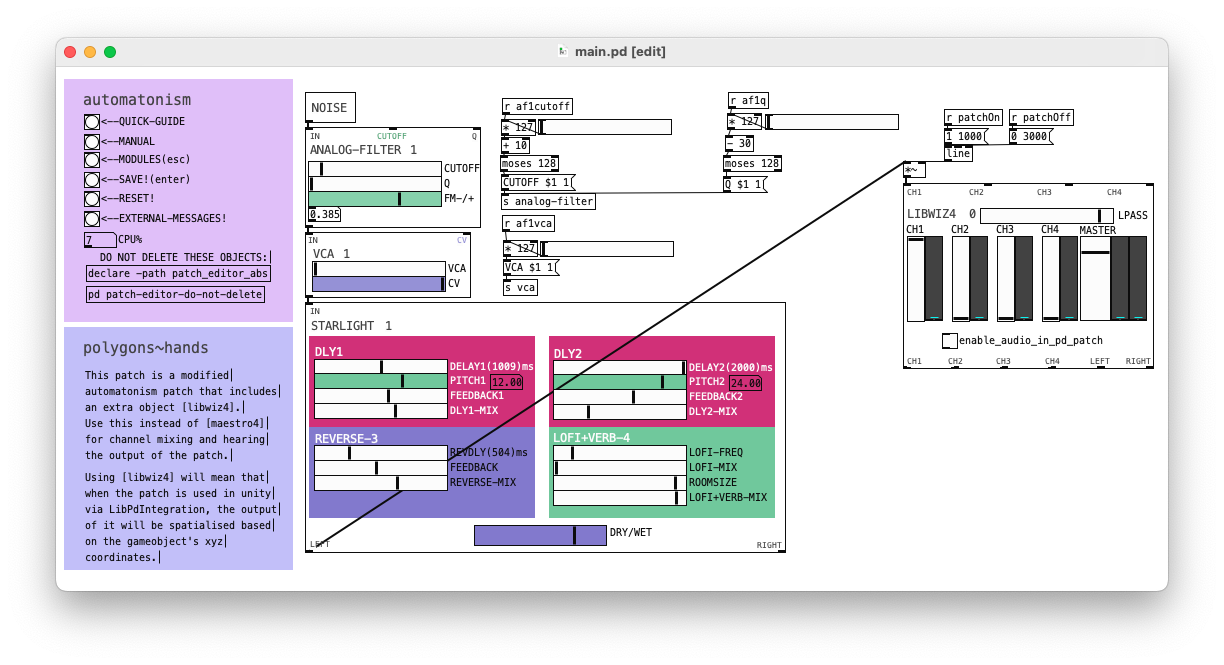
\includegraphics[angle=90,height=0.9\textheight]{07-polygons/polygons-hands-pd.png}
    \caption{The PureData patch for \textit{hands}}
    \label{fig: polygons-hands-pd}
\end{figure}

Together, and separately, \textit{ambi}, \textit{click+-}, and \textit{hands} provide a complex sound palette, explorable by the performer through non-linear combinations of hand gestures, body movements, and stances, that themselves invariably feed back into the decisions made to delve into and combine specific sounds. Visually, \textit{polygons\textasciitilde{}} draws on the pioneering 3D wire-frame AR systems of the 20th century such as the \textit{KARMA} system \citep{feiner1993} and Sutherland's \textit{Ultimate DIsplay} \citeyearpar{sutherland1968} (see: \autoref{fig: polygons-wireframes}), which were a design choice constrained by computational power at the time. This is juxtaposed by the fluid and visually complex behaviour of the thousands of multicoloured particles used by \textit{ambi}, and \textit{click+-}.

\begin{figure}
    \centering
    \captionsetup{justification=centering}
    \subcaptionbox{Through the `Head-Mounted Three Dimensional Display' \citep[in][]{sutherland1968}}[.32\linewidth]{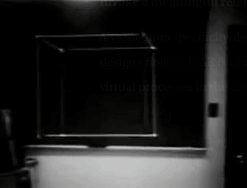
\includegraphics[height=3cm]{07-polygons/sutherland_68.png}}\label{fig: sutherland1968_in8}
    \hfill
    \subcaptionbox{Through the headset of the `KARMA' System \citep[in][]{feiner1993a}}[.32\linewidth]{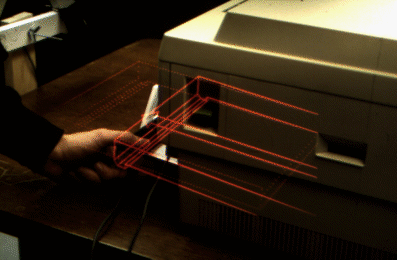
\includegraphics[height=3cm]{07-polygons/feiner_93_2.png}}\label{fig: feiner93_in8}
    \hfill
    \subcaptionbox{Through the viewport of `Virtual Sculpture' \citep[from][]{shaw1981}}[.32\linewidth]{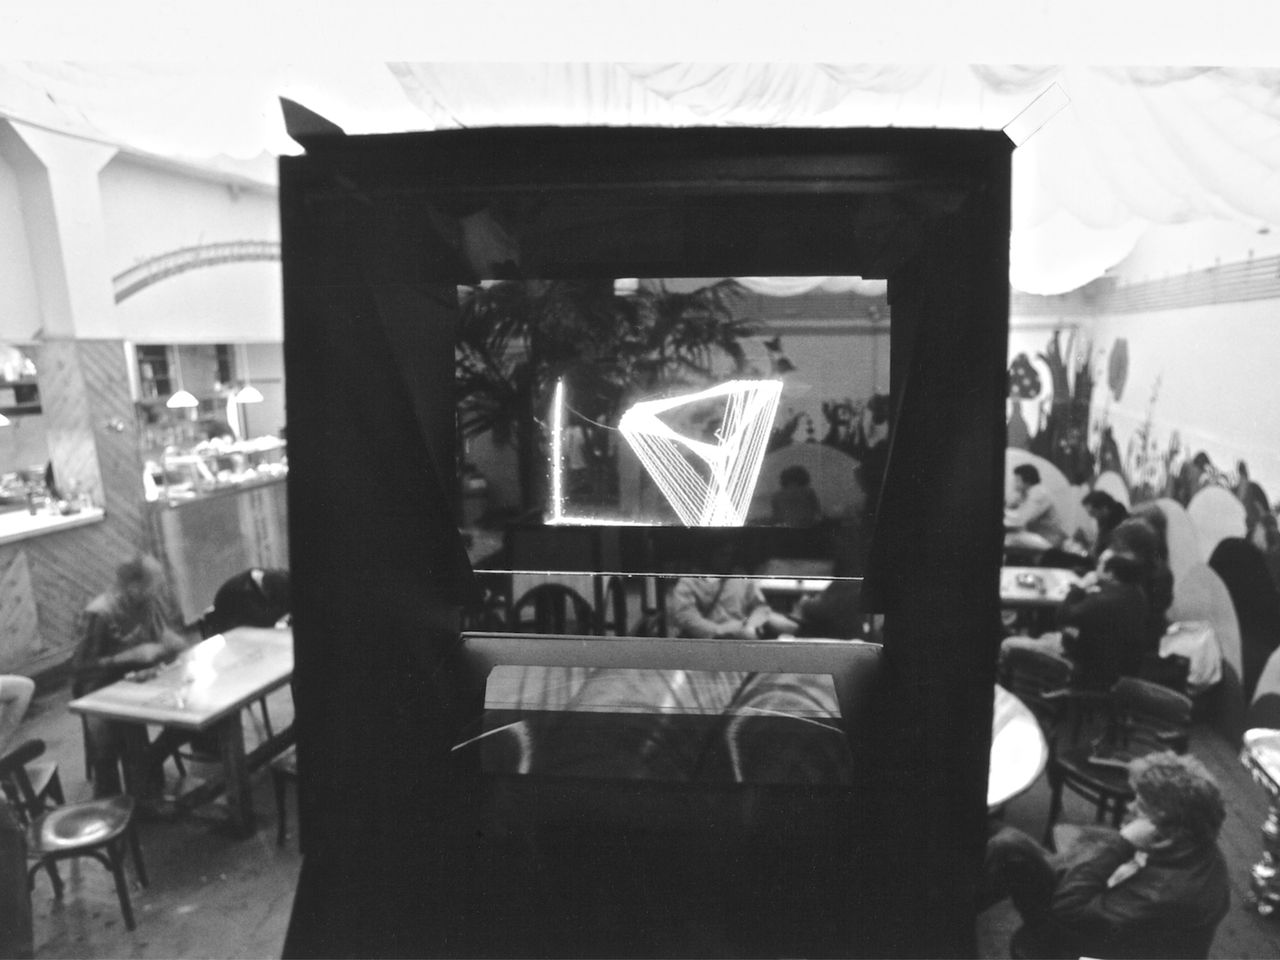
\includegraphics[height=3cm]{07-polygons/shaw1981.jpg}}\label{fig: shaw1981}
    \caption{Wire-frame influences for the polygons\textasciitilde{} instruments}
    \label{fig: polygons-wireframes}
\end{figure}


% --------------------------------------------------------------------------- %
\section{The Performance of \textit{polygons\textasciitilde{}}}\label{sec: polygons-performances}
\subsection{\textit{polygons\textasciitilde{}}Technical Setup}\label{sec: polygons-performances-setup}
From a system design perspective, as with any instrument, the importance of the performer's aesthetic experience as described the the previous section is indubitable; most of the software and hardware I had used in the development of \textit{polaris\textasciitilde{}} was readily transferable to the context of performance. There was no need to change from the combination of PureData, LibPdIntegration, and Unity. However, when considering the design of an AR experience \textit{as} performance, there began to surface new design considerations that needed answers:
\begin{itemize}
    \item \textit{By what means could I invite an audience into the hybrid space I was creating with \textit{polygons\textasciitilde{}}?} 
    \item \textit{What elements of my experience would / could be shared with an audience?} 
    \item \textit{How could I go about performing an experience that I was, by now, intimately aware of, but would be difficult without context for an audience to understand?} 
\end{itemize}
Due to time constraints, the performance system I decided on was fairly simple. For translating my visual experience (I deemed this necessary for the audience to understand my gestures and their links to musical outcomes) I would project the real-time hybrid composite feed (made up of a black and white video feed from one of the head-mounted sensors on the headset with an overlay of the Unity scene) on the wall behind me. For the audio, I replaced my bone-conduction headphones (sacrificing some of my own 3D audio immersion) with the PA system of the venue. The panning would be reversed so that my gestures and movements would translate realistically to the audiences auditory perspective, i.e. the movement of my hand during the performance of \textit{hands} across my body from left to right would transfer to the sound panning house-right to house-left rather than stage-left to stage-right.

\subsection{The Rosehill - February 2022}\label{sec: polygons-performances-rosehill}
\textit{polygons\textasciitilde{}} was developed for a performance as part of the seventh Experimental Music Technologies (emute) Lab \href{http://www.emutelab.org/blog/emutelab6}{showcase} at The Rosehill - an independent venue, recording studio, label, creative hub, and co-working space run by artists and musicians. The recording of the performance is hosted online, and can be found on the \textit{polygons\textasciitilde{}} \href{https://github.com/sambilbow/polygons}{GitHub repository}. The Rosehill performance was the first time I had immersed myself in the \textit{polygons\textasciitilde{}} system for an extended period of time; I had held off extended use of the system during prototyping the instruments. This lead to an authentic exploration and improvisation of the material, embodied, and spatial affordances of the three instruments, \textit{ambi}, \textit{click+-}, and \textit{hands}. The combination of sharing the audiovisual elements of my experience, auditory immersion of the audience, and performing through improvisation, led to an intimate performance. In itself, this decision was also an improvisation, I had not practiced or rehearsed, and this was my first performance of a non-traditional instrument. This took the form of me taking it upon myself to `showcase' the instruments to the audience, through a kind of theatrical and gestural dance that the audience were invited to be part of. 

One issue I hadn't anticipated was strobe caused by feedback between the visuals behind me and the sensor cameras in the headset when I stood in the throw of projector. This combined with the otherwise darkness of the room lead to a few moments where the sensors on the headset momentarily lost calibration, moving the Unity scene contents slightly. Whilst I (and study participants) had experienced this during \hyperref[sec: polaris-feedback-adoption-alignment]{\textit{polaris\textasciitilde{}}}, due to the confines of the stage, and the wall behind me, this did present slightly more of a problem and limited my performance space somewhat. For example, when \textit{click-} moved behind the wall, forcing me to stand flush with the wall and try very hard to take it out (\href{https://youtu.be/9IErsDvhXjM?t=210}{03:30}). This wrangling between the virtual and physical space presented itself as a comedic moment for the audience, and was a moment of where the mechanics of the hybrid space became obvious, and relatable despite the distance between the audience and my own understanding and experience of AR. Overall though, the performance, despite its hitches was received extremely well, with members of the audience afterwards exclaiming that they'd never seen any such kind of performance. 

\subsection{Showcase at the ACCA - June 2022}\label{sec: polygons-performances-acca}
\textit{polygons\textasciitilde{}} was performed three months later at an end-of-year departmental showcase at the Attenborough Centre for the Creative Arts (see \autoref{fig: polygons-acca}). The space here was much larger, allowing me more space to explore (although still limited by the length of the headset cable - 2.5 metres), it reduced the chance of the aforementioned strobe, which made the sensor alignment more stable.

\begin{figure}
    \centering
    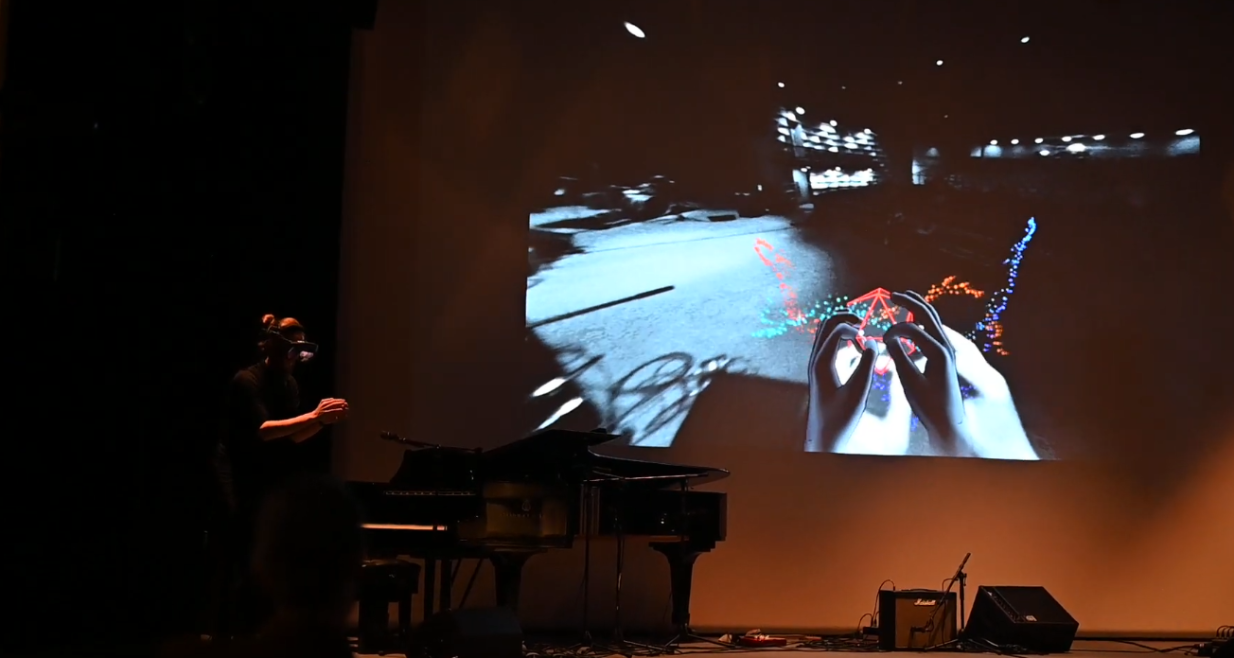
\includegraphics[width=0.7\linewidth]{07-polygons/polygons-acca.png}
    \caption{\textit{polygons\textasciitilde{}} performance at the ACCA}
    \label{fig: polygons-acca}
\end{figure}

\subsection{Demonstrations - May \& June 2022}\label{sec: polygons-performances-demos}
For furthering understanding of AR as a medium for artistic and musical practice, as well as for providing novel experiences to those who hadn't experienced AR yet, \textit{polygons\textasciitilde{}} was made open for students and faculty to perform and experience as part of the first MAH Doctoral Conference. It was also open for experience as part of the SHL Make \& Create day, on the 25th of May, and 9th of June 2022 respectively.

These sessions provided a chance to glean some face-to-face informal feedback on the design, rationale, and sound-world of \textit{polygons\textasciitilde{}}. Not to mention, it was an exercise in seeing second hand the amount of embodied knowledge, and skilful AR know-how I had accumulated with the system I had used for 18 months by this point. Those experiencing XR for the first time definitely struggled more with the gestures needed to move, resize, and interact with the three instruments.



% --------------------------------------------------------------------------- %
\section{The Future of AR Sound ARt Performance}
From the performance of \textit{polygons\textasciitilde{}}, it became clear to me that AR within a musical performance practice can be an effective medium for the creation of novel aesthetic experiences for performer \textit{and} audience. However, improvements could be made to the process of `inviting' the audience into the performer's hybrid space. \textit{polygons\textasciitilde{}} in this regard, was fairly unpolished, even for a first performance - and I imagine the audience felt as if they were `witnessing' rather than `experiencing' with me. Therefore, I envisage the challenges for future AR musical performances in my own, and in the broader community's practices, lying in the development of immersive audience experiences.

 With the exception of the incredible work by Amy Brandon using the METAVision headset \citeyearpar{brandon2018}, I have been hard-pressed to find other live audiovisual performances that specifically appropriate AR \textit{headsets} as their actual medium of performance. Despite there being an array of cutting edge performances that use AR technologies in their execution, it is extremely new as a research area, with a lot of exploration and research to be done. Like in most aspects, due to the amount of funding and earlier research focus, VR has been an area where artistic and musical performance has flourished in the last 20 years, with early pioneers \citep{davies2004} paving the way for the consideration of the body in immersive 3D space. \textit{polygons\textasciitilde{}} could be closely linked to contemporary VR visual art making practices, where artists sculpt, paint, and draw in 3D in an infinite world canvas \citep{summers2019}. AR musical performance however, is beginning to gain traction, with participatory installations \citep{chevalier2018},  projection-based performances \citep{quay2016,berthaut2016,robinson2020}, tangible AR projects \citep{zamborlin2018}, and real-time notation techniques \citep{santini2020,santini2022}. 

As found in the field of spatial acousmatic performance \citep{sharma2015}, a clear vocabulary ought be developed here due to the wide disciplinary scope of the technologies, aesthetics, and modes of performance explored. Indeed, the public perception of `AR performances' has typically come to describe the use of AR as the \textit{medium of playback} -- replacing the 2D screen with an immersive 3D viewing/listening of a live or pre-recorded musical experience -- rather than the \textit{medium of performance}.

\textit{polygons\textasciitilde{}}, like any prototype instrument or performance, has therefore asked more questions that it has answered. Concerning the future of AR musical performance, the present thesis proposes the following questions as potential research avenues:
\begin{itemize}
    \item Can we avoid `spectacle' of AR? How else can we meaningfully engage audiences who are new to AR?
    \item How can we invite the audience into AR musical performance more effectively?
    \item Is wearing more technology necessarily the best avenue for a focus on embodied performance?
    \item What would an AR ensemble look, sound, and feel like for both performer and audience?
    \item Could AR be appropriated for real-time networked performance of physically separate spaces?
\end{itemize}